\documentclass{../../slides-style}

\slidetitle{Продолжение про F\#}{20.02.2025}

\begin{document}
    
    \begin{frame}[plain]
        \titlepage
    \end{frame}

    \section{Юнит-тестирование}

    \begin{frame}
        \frametitle{Юнит-тестирование в F\#}
        \begin{itemize}
            \item Работают все дотнетовские библиотеки (NUnit, MsTest и т.д.)
            \item Есть обёртки, делающие код тестов более \enquote{функциональным} (FsUnit)
            \item Есть чисто F\#-овские штуки: FsCheck, Unquote 
            \begin{itemize}
                \item на самом деле, не совсем F\#-овские, но в C\# такого нет
                \item на самом деле, есть, это называется property-based testing и считается передовой техникой тестирования, в F\# было всегда
            \end{itemize}
        \end{itemize}
    \end{frame}

    \begin{frame}[fragile]
        \frametitle{FsUnit, пример}
        \begin{minted}{fsharp}
module ``Project Euler - Problem 1`` =
    open NUnit.Framework
    open FsUnit

    let GetSumOfMultiplesOf3And5 max =
        seq{3 .. max - 1} 
        |> Seq.fold(fun acc number ->
                    (if (number % 3 = 0 || number % 5 = 0) then
                         acc + number else acc)) 0

    [<Test>]
    let ``Sum of multiples of 3 and 5 to 10 should return 23`` () =
        GetSumOfMultiplesOf3And5(10) |> should equal 23
        \end{minted}
    \end{frame}

    \begin{frame}[fragile]
        \frametitle{FsUnit, матчеры}
        \begin{minted}{fsharp}
1 |> should equal 1
1 |> should not' (equal 2)
10.1 |> should (equalWithin 0.1) 10.11
"ships" |> should startWith "sh"
"ships" |> should not' (endWith "ss")
"ships" |> should haveSubstring "hip"
[1] |> should contain 1
[] |> should not' (contain 1)
anArray |> should haveLength 4

(fun () -> failwith "BOOM!" |> ignore) 
    |> should throw typeof<System.Exception>

shouldFail (fun () -> 5/0 |> ignore)
        \end{minted}
    \end{frame}

    \begin{frame}[fragile]
        \frametitle{FsUnit, ещё матчеры}
        \begin{minted}{fsharp}
true |> should be True
false |> should not' (be True)
"" |> should be EmptyString
null |> should be Null

anObj |> should not' (be sameAs otherObj)

11 |> should be (greaterThan 10)
10.0 |> should be (lessThanOrEqualTo 10.1)

0.0 |> should be ofExactType<float>
1 |> should not' (be ofExactType<obj>)
        \end{minted}
    \end{frame}

    \begin{frame}[fragile]
        \frametitle{FsUnit, и ещё матчеры}
        \begin{minted}{fsharp}
Choice<int, string>.Choice1Of2(42) |> should be (choice 1)

"test" |> should be instanceOfType<string>
"test" |> should not' (be instanceOfType<int>)

2.0 |> should not' (be NaN)

[1; 2; 3] |> should be unique

[1; 2; 3] |> should be ascending
[1; 3; 2] |> should not' (be ascending)
[3; 2; 1] |> should be descending
[3; 1; 2] |> should not' (be descending)
        \end{minted}
    \end{frame}

    \begin{frame}[fragile]
        \frametitle{Значения в модулях не инициализируются!}
        \framesubtitle{Как внезапно прострелить себе ногу}
        Main.fs:
        \begin{minted}{fsharp}
let value = [1]
        \end{minted}
        \vspace{5mm}
        Test.fs:
        \begin{minted}{fsharp}
[<Test>]
let Test () =
    Assert.AreEqual([1], Main.value)
        \end{minted}
        \vspace{5mm}
        Вывод:
        \begin{minted}{text}
Failed Test1 [24 ms]
Error Message:
   Expected: < 1 >
But was:  null     
        \end{minted}
    \end{frame}

    \begin{frame}[fragile]
        \frametitle{FsCheck}
        \begin{minted}{fsharp}
open FsCheck

let revRevIsOrig (xs:list<int>) = List.rev(List.rev xs) = xs

Check.Quick revRevIsOrig
// Ok, passed 100 tests.

let revIsOrig (xs:list<int>) = List.rev xs = xs
Check.Quick revIsOrig
// Falsifiable, after 2 tests (2 shrinks) (StdGen (338235241,296278002)):
// Original:
// [3; 0]
// Shrunk:
// [1; 0]
        \end{minted}
        Для интеграции с FsUnit используйте Check.QuickThrowOnFailure
    \end{frame}

    \begin{frame}[fragile]
        \frametitle{Unquote}
        Вообще интерпретатор F\#-а, очень полезный для тестирования:
        \begin{minted}{fsharp}
[<Test>]
let ``Unquote demo`` () =
    test <@ ([3; 2; 1; 0] |> List.map ((+) 1)) = [1 + 3..1 + 0] @>

// ([3; 2; 1; 0] |> List.map ((+) 1)) = [1 + 3..1 + 0]
// [4; 3; 2; 1] = [4..1]
// [4; 3; 2; 1] = []
// false
        \end{minted}
    \end{frame}

    \begin{frame}[fragile]
        \frametitle{Foq}
        Ну и, конечно же, mock-объекты:
        \begin{minted}{fsharp}
[<Test>]
let ``Foq demo`` () =
    let mock = Mock<System.Collections.Generic.IList<int>>()
                .Setup(fun x -> <@ x.Contains(any()) @>).Returns(true)
                .Create()

    mock.Contains 1 |> Assert.True
        \end{minted}
    \end{frame}

    \section{Каррирование}

    \begin{frame}[fragile]
        \frametitle{Каррирование, частичное применение}
        \begin{minted}{fsharp}
let shift (dx, dy) (px, py) = (px + dx, py + dy)
let shiftRight = shift (1, 0)
let shiftUp = shift (0, 1)
let shiftLeft = shift (-1, 0)
let shiftDown = shift (0, -1)
        \end{minted}
        \begin{alertblock}{F\# Interactive}
            \begin{minted}{fsharp}
> shiftDown (1, 1);;
val it : int * int = (1, 0)
            \end{minted}
        \end{alertblock}
    \end{frame}

    \begin{frame}[fragile]
        \frametitle{Зачем --- функции высших порядков}
        \begin{minted}{fsharp}
let lists = [[1; 2]; [1]; [1; 2; 3]; [1; 2]; [1]]
let lengths = List.map List.length lists
        \end{minted}
        или
        \begin{minted}{fsharp}
let lists = [[1; 2]; [1]; [1; 2; 3]; [1; 2]; [1]]
let squares = List.map (List.map (fun x -> x * x)) lists
        \end{minted}
        \vspace{3mm}
        Функции стандартной библиотеки стараются принимать список последним, для каррирования
    \end{frame}

    \section{Композиция}

    \begin{frame}[fragile]
        \frametitle{Оператор $|>$}
        \framesubtitle{Pipe forward}
        \begin{minted}{fsharp}
let (|>) x f = f x
        \end{minted}

        \begin{minted}{fsharp}
let sumFirst3 ls = ls |> Seq.take 3 |> Seq.fold (+) 0
        \end{minted}
        вместо
        \begin{minted}{fsharp}
let sumFirst3 ls= Seq.fold (+) 0 (Seq.take 3 ls)
        \end{minted}
    \end{frame}

    \begin{frame}[fragile]
        \frametitle{Оператор $>>$}
        \framesubtitle{Композиция}
        \begin{minted}{fsharp}
let (>>) f g x = g (f x)
        \end{minted}
        \begin{minted}{fsharp}
let sumFirst3 = Seq.take 3 >> Seq.fold (+) 0
let result = sumFirst3 [1; 2; 3; 4; 5]
        \end{minted}
    \end{frame}

    \begin{frame}[fragile]
        \frametitle{Операторы $<|$ и $<<$}
        \framesubtitle{Pipe-backward и обратная композиция}
        \begin{minted}{fsharp}
let (<|) f x = f x
let (<<) f g x = f (g x)
        \end{minted}
        Зачем? Чтобы не ставить скобки:
        \begin{minted}{fsharp}
printfn "Result = %d" <| factorial 5
        \end{minted}
    \end{frame}

    \section{.NET}

    \begin{frame}[fragile]
        \frametitle{Использование библиотек .NET}
        \begin{scriptsize}
            \begin{minted}{fsharp}
open System.Windows.Forms

let form = new Form(Visible = false, TopMost = true, Text = "Welcome to F#")
let textB = new RichTextBox(Dock = DockStyle.Fill, Text = "Some text")
form.Controls.Add(textB)

open System.IO
open System.Net

/// Get the contents of the URL via a web request
let http(url: string) =
    let req = System.Net.WebRequest.Create(url)
    let resp = req.GetResponse()
    let stream = resp.GetResponseStream()
    let reader = new StreamReader(stream)
    let html = reader.ReadToEnd()
    resp.Close()
    html

textB.Text <- http("http://www.google.com")

form.ShowDialog () |> ignore
            \end{minted}
        \end{scriptsize}
    \end{frame}

    \section{Сопоставление шаблонов}
    
    \begin{frame}[fragile]
        \frametitle{Сопоставление шаблонов}
        \begin{minted}{fsharp}
let urlFilter url agent =
    match (url, agent) with
    | "http://www.google.com", 99 -> true
    | "http://www.yandex.ru" , _ -> false
    | _, 86 -> true
    | _ -> false
        \end{minted}

        \begin{minted}{fsharp}
let sign x =
    match x with
    | _ when x < 0 -> -1
    | _ when x > 0 -> 1
    | _ -> 0
        \end{minted}
    \end{frame}

    \begin{frame}[fragile]
        \frametitle{F\# --- не Prolog}
        Не получится писать так:
        \begin{minted}{fsharp}
let isSame pair =
    match pair with
    | (a, a) -> true
    | _ -> false
        \end{minted}
        Нужно так:
        \begin{minted}{fsharp}
let isSame pair =
    match pair with
    | (a, b) when a = b -> true
    | _ -> false
        \end{minted}
    \end{frame}

    \begin{frame}
        \frametitle{Какие шаблоны бывают}
        \begin{small}
            \begin{tabu} {| X[0.9 l p] | X[1 l p] | X[1 l p] |}
                \tabucline-
                Синтаксис                               & Описание                  & Пример                  \\
                \tabucline-
                \everyrow{\tabucline-}
                $(pat, \ldots, pat)$                    & Кортеж                    & $(1, 2, (``3``, x))$    \\
                $[pat; \ldots; pat]$                    & Список                    & $[x; y; 3]$             \\
                $pat :: pat$                            & cons                      & $h :: t$                \\
                $pat\ |\ pat$                           & "Или"                     & $[x]\ |\ [``X``\ ;\ x]$ \\
                $pat\ \&\ pat$                          & "И"                       & $[p] \& [(x, y)]$       \\
                $pat\ as\ id$                           & Именованный шаблон        & $[x]\ as\ inp$          \\
                $id$                                    & Переменная                & $x$                     \\
                $\_$                                    & Wildcard (что угодно)     & $\_$                    \\
                литерал                                 & Константа                 & $239, DayOfWeek.Monday$ \\
                $:?\ type$                              & Проверка на тип           & $:?\ string$            \\
            \end{tabu}
        \end{small}
    \end{frame}

    \section{Последовательности}
    
    \begin{frame}[fragile]
        \frametitle{Последовательности}
        \framesubtitle{Ленивый тип данных}
        \begin{minted}{fsharp}
seq {0 .. 2}
seq {1I .. 1000000000000I}
        \end{minted}

        \begin{minted}{fsharp}
open System.IO
let rec allFiles dir =
    Seq.append
    (dir |> Directory.GetFiles)
    (dir |> Directory.GetDirectories 
         |> Seq.map allFiles 
         |> Seq.concat)
        \end{minted}
    \end{frame}

    \begin{frame}
        \frametitle{Типичные операции с последовательностями}
        \begin{small}
            \begin{tabu} {| X[0.5 l p] | X[1 l p] |}
                \tabucline-
                Операция                               & Тип                    \\
                \tabucline-
                \everyrow{\tabucline-}
                Seq.append                    & $\#seq<'a> \to \#seq<'a> \to seq<'a>$ \\
                Seq.concat                    & $\#seq<\#seq<'a>> \to seq<'a>$ \\
                Seq.choose                    & $('a \to 'b\ option) \to \#seq<'a> \to seq<'b>$ \\
                Seq.empty                     & $seq<'a>$ \\
                Seq.map                       & $('a \to 'b) \to \#seq<'a> \to \#seq<'b>$ \\
                Seq.filter                    & $('a \to bool) \to \#seq<'a> \to seq<'a>$ \\
                Seq.fold                      & $('s \to 'a \to 's) \to 's \to seq<'a> \to 's$ \\
                Seq.initInfinite              & $(int \to 'a) \to seq<'a>$ \\
            \end{tabu}
        \end{small}
    \end{frame}

    \section{Записи}
    
    \begin{frame}[fragile]
        \frametitle{Записи}
        \begin{minted}{fsharp}
type Person =
    { Name: string
      DateOfBirth: System.DateTime }
        \end{minted}

        \begin{minted}{fsharp}
{ Name = "Bill"
  DateOfBirth = new System.DateTime(1962, 09, 02) }

{ new Person
  with Name = "Anna"
  and DateOfBirth = new System.DateTime(1968, 07, 23) }
        \end{minted}
    \end{frame}

    \begin{frame}[fragile]
        \frametitle{Деконструкция}
        \begin{minted}{fsharp}
let person = { Name = "Anna"
               DateOfBirth = new System.DateTime(1968, 07, 23) }

let { Name = name; DateOfBirth = date} = person

// деконструкция в параметре функции f
let f { Name = name; DateOfBirth = date} =  ..
        \end{minted}
    \end{frame}

    \begin{frame}[fragile]
        \frametitle{Анонимные записи}
        \begin{minted}{fsharp}
let person = {| Name = "Anna"; DateOfBirth = DateTime(1968, 07, 23) |}
        \end{minted}
        \begin{itemize}
            \item Могут возвращаться из функций (в отличие от анонимных объектов в C\#)
            \item Имеют структурное равенство и сравнение
                \begin{minted}{fsharp}
                {| a = 2 |} > {| a = 1 |} // true
                \end{minted}
            \item Не могут участвовать в сопоставлении с шаблоном
        \end{itemize}
    \end{frame}

    \section{Размеченные объединения}
    
    \begin{frame}[fragile]
        \frametitle{Размеченные объединения}
        \framesubtitle{Discriminated unions}
        \begin{minted}{fsharp}
type Route = int
type Make = string
type Model = string

type Transport =
    | Car of Make * Model
    | Bicycle
    | Bus of Route

let bus = Bus(420)
        \end{minted}
    \end{frame}

    \begin{frame}[fragile]
        \frametitle{Известные примеры}
        \begin{minted}{fsharp}
type 'a option =
    | None
    | Some of 'a
        \end{minted}

        \vspace{5mm}
        \begin{minted}{fsharp}
type 'a list =
    | ([])
    | (::) of 'a * 'a list
        \end{minted}
    \end{frame}

    \begin{frame}[fragile]
        \frametitle{Использование размеченных объединений}
        \begin{minted}{fsharp}
type IntOrBool = I of int | B of bool
let i = I 99
let b = B true
        \end{minted}
        
        \begin{minted}{fsharp}
type C = Circle of int | Rectangle of int * int

[1..10]
|> List.map Circle

[1..10]
|> List.zip [21..30]
|> List.map Rectangle
        \end{minted}
    \end{frame}

    \begin{frame}[fragile]
        \frametitle{Использование в match}
        \begin{minted}{fsharp}
type Tree<'a> =
    | Tree of 'a * Tree<'a> * Tree<'a>
    | Tip of 'a

let rec size tree =
    match tree with
    | Tree(_, l, r) -> 1 + size l + size r
    | Tip _ -> 1
        \end{minted}
    \end{frame}

    \begin{frame}[fragile]
        \frametitle{Пример}
        \framesubtitle{Дерево разбора логического выражения}
        \begin{minted}{fsharp}
type Proposition =
    | True
    | And of Proposition * Proposition
    | Or of Proposition * Proposition
    | Not of Proposition

let rec eval (p: Proposition) =
    match p with
    | True -> true
    | And(p1, p2) -> eval p1 && eval p2
    | Or (p1, p2) -> eval p1 || eval p2
    | Not(p1) -> not (eval p1)

printfn "%A" <| eval (Or(True, And(True, Not True)))
        \end{minted}
    \end{frame}

    \begin{frame}[fragile]
        \frametitle{Взаимосвязанные типы}
        \begin{minted}{fsharp}
type Node =
    { Name : string;
      Links : Link list }
and Link =
    | Dangling
    | Link of Node
        \end{minted}
    \end{frame}

    \subsection{Одноэлементные объединения}

    \begin{frame}[fragile]
        \frametitle{Одноэлементные объединения, без}
        \begin{minted}{fsharp}
type CustomerId = int  // синоним типа
type OrderId = int  // ещё один синоним типа

let printOrderId (orderId: OrderId) =
  printfn "The orderId is %i" orderId

let customerId = 1  
printOrderId customerId  // Печаааль
        \end{minted}
    \end{frame}

    \begin{frame}[fragile]
        \frametitle{Одноэлементные объединения, с}
        \begin{minted}{fsharp}
type CustomerId = CustomerId of int  // размеченное объединение 
type OrderId = OrderId of int // ещё одно

let printOrderId (OrderId orderId) = // деконструкция в параметре
    printfn "The orderId is %i" orderId

let customerId = CustomerId 1
printOrderId customerId  // Ошибка компиляции
        \end{minted}
    \end{frame}

    \section{Хвостовая рекурсия}

    \begin{frame}[fragile]
        \frametitle{Факториал без хвостовой рекурсии}
        \begin{minted}{fsharp}
let rec factorial x =
    if x <= 1
    then 1 
    else x * factorial (x - 1)
        \end{minted}

        \begin{minted}{fsharp}
let rec factorial x =
    if x <= 1
    then
        1
    else
        let resultOfRecusion = factorial (x - 1)
        let result = x * resultOfRecusion
        result
        \end{minted}
    \end{frame}

    \begin{frame}[fragile]
        \frametitle{Факториал с хвостовой рекурсией}
        \begin{minted}{fsharp}
let factorial x =
    let rec tailRecursiveFactorial x acc =
        if x <= 1 then
            acc
        else
            tailRecursiveFactorial (x - 1) (acc * x)
    tailRecursiveFactorial x 1
        \end{minted}
    \end{frame}
    
    \begin{frame}[fragile]
        \frametitle{После декомпиляции в C\#}
        \begin{alertblock}{C\#}
            \begin{minted}{csharp}
public static int tailRecursiveFactorial(int x, int acc)
{
    while (true)
    {
        if (x <= 1)
        {
            return acc;
        }
        acc *= x;
        x--;
    }
}
            \end{minted}
        \end{alertblock}
    \end{frame}

    \begin{frame}[fragile]
        \frametitle{Паттерн ``Аккумулятор''}
        \begin{minted}{fsharp}
let rec map f list =
    match list with
    | [] -> []
    | hd :: tl -> (f hd) :: (map f tl)

let map f list =
    let rec mapTR f list acc =
        match list with
        | [] -> acc
        | hd :: tl -> mapTR f tl (f hd :: acc)
    mapTR f (List.rev list) []
        \end{minted}
    \end{frame}

    \section{CPS}

    \begin{frame}[fragile]
        \frametitle{Continuation Passing Style}
        \framesubtitle{Аккумулятор --- функция}
        \begin{columns}
            \begin{column}{0.7\textwidth}
                \begin{minted}{fsharp}
let printListRev list =
    let rec printListRevTR list cont =
        match list with
        | [] -> cont ()
        | hd :: tl ->
            printListRevTR tl (fun () -> 
                printf "%d " hd; cont () )
    printListRevTR list (fun () -> printfn "Done!")
                \end{minted}
            \end{column}
            \begin{column}{0.3\textwidth}
                \begin{center}
                    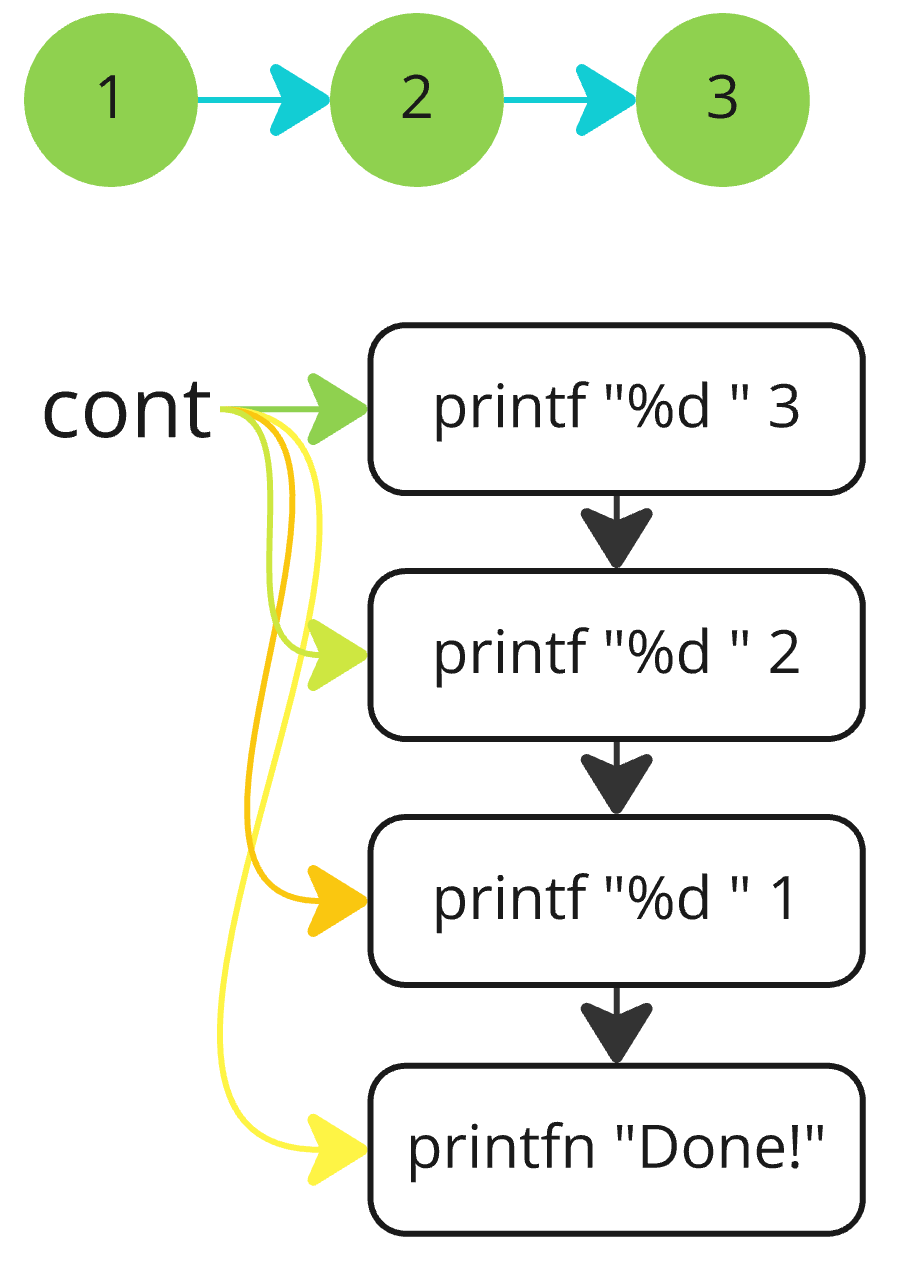
\includegraphics[width=\textwidth]{continuation.png}
                \end{center}
            \end{column}
        \end{columns}
    \end{frame}

    \begin{frame}[fragile]
        \frametitle{Обход дерева}
        \frametitle{Когда всё не так просто}
        \begin{minted}{fsharp}
type ContinuationStep<'a> =
    | Finished
    | Step of 'a * (unit -> ContinuationStep<'a>)

let rec linearize binTree cont =
    match binTree with
    | Empty -> cont()
    | Node(x, l, r) ->
        Step(x, (fun () -> linearize l (fun () -> 
                           linearize r cont)))
        \end{minted}
    \end{frame}

    \begin{frame}
        \frametitle{Что происходит}
        \begin{center}
            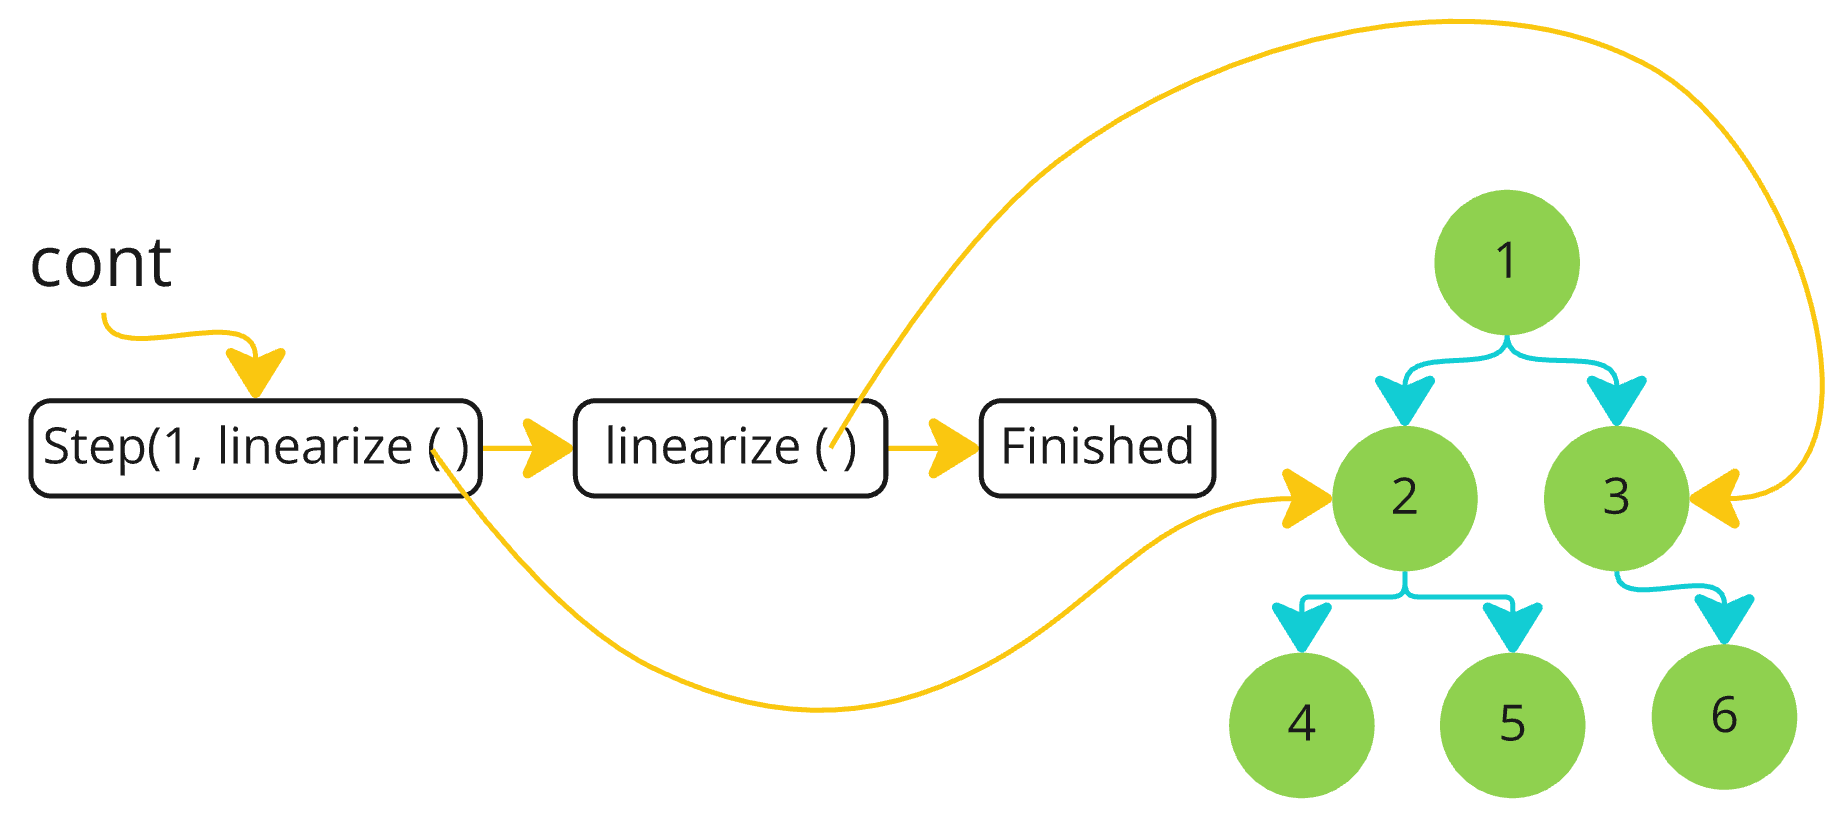
\includegraphics[width=0.95\textwidth]{treeLinearization.png}
        \end{center}
    \end{frame}

    \begin{frame}[fragile]
        \frametitle{Обход дерева}
        \frametitle{Собственно, обход}
        \begin{minted}{fsharp}
let iter f binTree =
    let steps = linearize binTree (fun () -> Finished)

    let rec processSteps step =
        match step with
        | Finished -> ()
        | Step(x, getNext) -> 
            f x
            processSteps (getNext())
    
    processSteps steps
        \end{minted}
    \end{frame}

    \begin{frame}
        \frametitle{Пример шага обхода}
        \begin{center}
            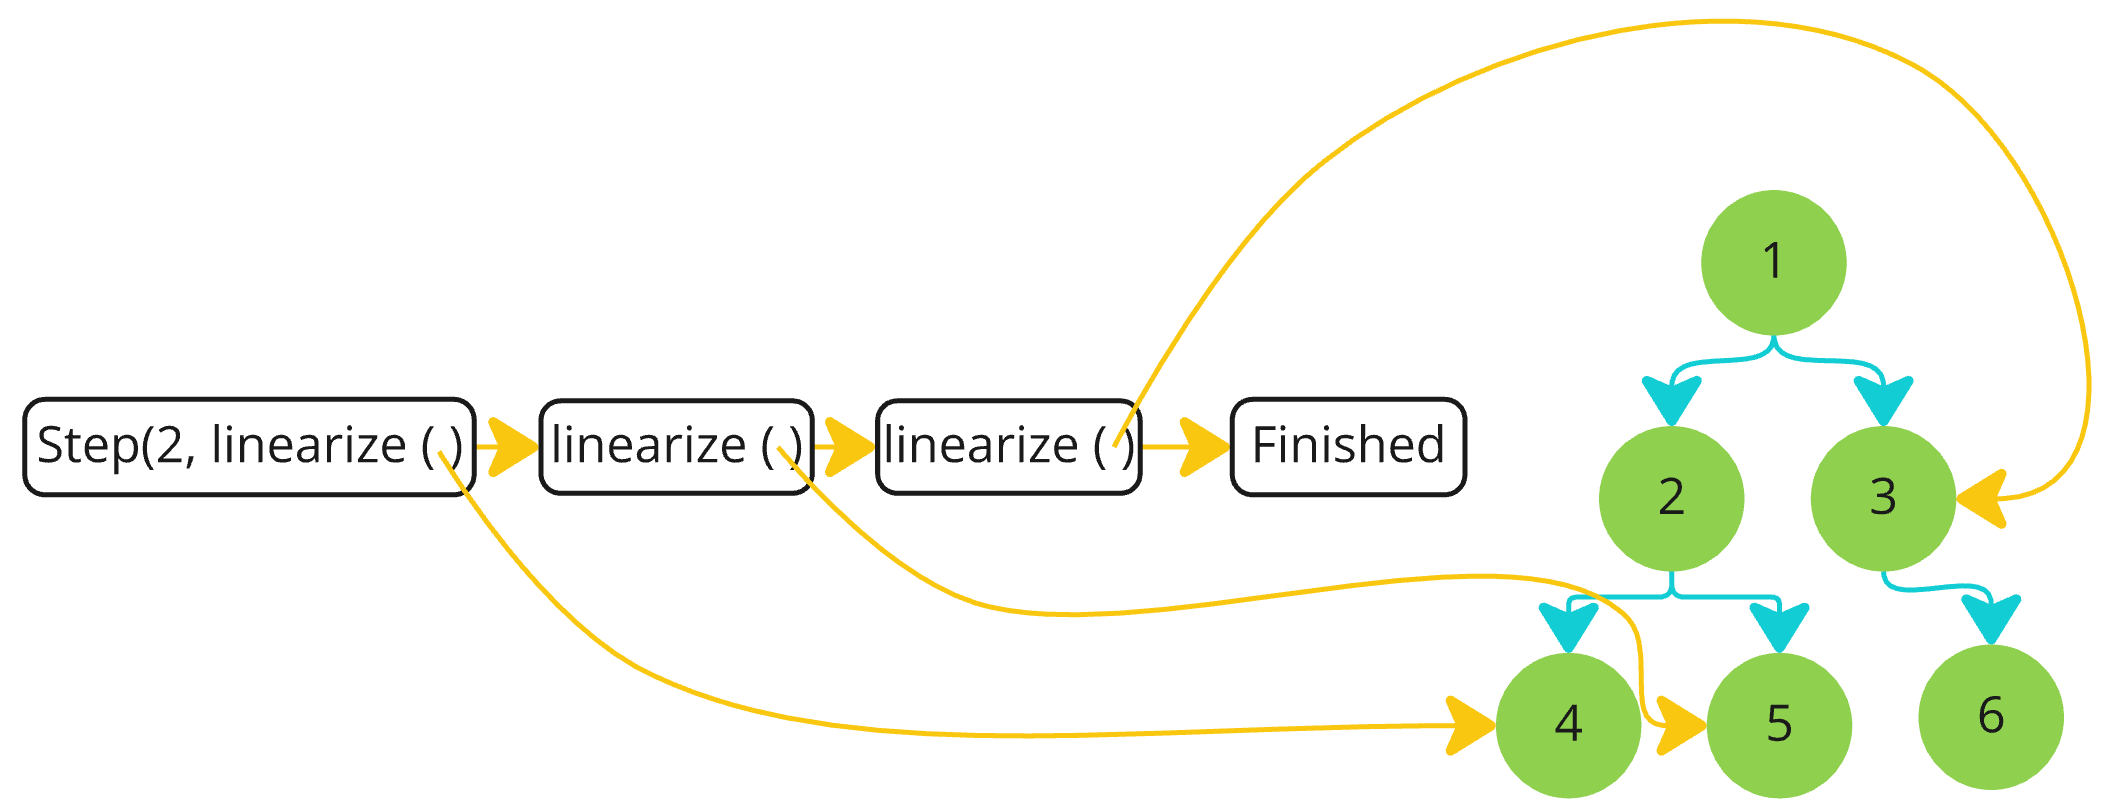
\includegraphics[width=0.95\textwidth]{treeLinearizationStep.png}
        \end{center}
    \end{frame}

\end{document}